\documentclass{article}
\usepackage[utf8]{inputenc}
\documentclass[preprint,authoryear]{elsarticle}
%\usepackage[english]{babel}
%\usepackage[utf8x]{inputenc}
\usepackage{fullpage}
\usepackage{subcaption} %Subfigure
%\usepackage{subfigure} %Subfigure
\usepackage{pifont}
\usepackage{latexsym}
\usepackage{mathrsfs}
\usepackage{amssymb,amsbsy}
\usepackage{amsmath}     
\usepackage{amsfonts}
\usepackage{graphicx}
\usepackage{tcolorbox}
\usepackage[colorinlistoftodos]{todonotes}
\usepackage{varwidth}
%\usepackage{authblk}
\usepackage{algorithm}
\usepackage[ruled,vlined]{algorithm2e}
\usepackage{algorithmic}
\usepackage{lmodern}
\usepackage{natbib}
\usepackage{mathtools}      
\usepackage[titletoc]{appendix}
%\usepackage{titlesec}       
\usepackage{titletoc}
\usepackage{ntheorem}
\DeclareMathOperator{\Hessian}{Hess}

%\graphicspath{{Images/}}
\usepackage{graphicx}
\usepackage{epsfig}
%% The amssymb package provides various useful mathematical symbols
\usepackage{amssymb}
\usepackage{amsmath}  
\usepackage{float}
\newfloat{algorithm}{t}{lop}
\usepackage{lipsum}% http://ctan.org/pkg/lipsum
\usepackage{tikz}   %allows shapes of nodes
\usetikzlibrary{shapes,arrows}
%\usetikzlibrary{positioning,chains,fit,shapes,calc}
%\usetikzlibrary{trees} 
%\usepackage{tkz-graph}
\usetikzlibrary{positioning, automata}
\usepackage{makeidx}         % allows index generation
 \usepackage{blkarray}% http://ctan.org/pkg/blkarray
 \newcommand{\matindex}[1]{\mbox{\scriptsize#1}}% Matrix index
 \usepackage{dcolumn}
\newcolumntype{L}{D{.}{.}{1.1}}
\usepackage{multirow}% http://ctan.org/pkg/multirow
\usepackage{hhline}% http://ctan.org/pkg/hhline
\usepackage{caption}
%\captionsetup{labelsep=space,justification=justified,singlelinecheck=off}
 \usepackage{fancyhdr,graphicx,amsmath,amssymb}
%\usepackage[ruled,vlined]{algorithm2e}

%%%%%%%%%%%%%%%%%%%%%%%%%%%%
% Code Listing for Python code
\definecolor{codegreen}{rgb}{0,0.6,0}
\definecolor{codegray}{rgb}{0.5,0.5,0.5}
\definecolor{codepurple}{rgb}{0.58,0,0.82}
\definecolor{backcolour}{rgb}{0.95,0.95,0.92}

\usepackage{listings}
\include{pythonlisting}
\lstdefinestyle{mystyle}{
  backgroundcolor=\color{backcolour},   commentstyle=\color{codegreen},
  keywordstyle=\color{magenta},
  numberstyle=\tiny\color{codegray},
  stringstyle=\color{codepurple},
  basicstyle=\ttfamily\footnotesize,
  breakatwhitespace=false,         
  breaklines=true,                 
  captionpos=b,                    
  keepspaces=true,                 
  numbers=left,                    
  numbersep=5pt,                  
  showspaces=false,                
  showstringspaces=false,
  showtabs=false,                  
  tabsize=2
}

%"mystyle" code listing set
\lstset{style=mystyle}
 
\usepackage[bottom]{footmisc}% places footnotes at page bottom
\usepackage{algorithm, algpseudocode} 
\captionsetup{compatibility=false} 
\usepackage{listings}
\floatstyle{plain} % Box...
%\restylefloat{figure}% ...figure environment contents.






%for JSON
\usepackage{bera}% optional: just to have a nice mono-spaced font
\usepackage{listings}
\usepackage{xcolor}
\title{CES derivations}
\author{Poulami SArkar}
\date{December 2019}

\begin{document}

\maketitle
We intend to explore the global influence (internationality) of academic institutions in terms of non-local citations(global citations).  This can be of great interest to many potential students, academicians as well as researchers.  The influence of institutions over time and is a non-linear system and can incorporate chaos.  We posit a novel method to model this influence by using the Constant Elasticity of Substitution (CES) function optimized using the Particle swarm optimization algorithm(PSO) under chaotic conditions

section{The CES function}
In the extant literature,  convex optimization principle has been used in the recent past to solvefundamental problems in science.  Notwithstanding, optimization associated with technology relatedto performance in data centers and the problem of cost minimization remains an important issue.  Weare aware of the cross-effects of reducing the use of one factor vis-a-vis another and apply the CESproduction function to estimate the impact of reducing the cost of the contributing factors on revenuemaximization  at  the  data  centers.   It  is  well-known  that  CES  belongs  to  the  family  of  neoclassicalproduction functions and the CES production function for two inputs can be represented in the formbelow:


\begin{equation}          
Q(L,K)=(\alpha{K}^\rho+(1-\alpha)L^\rho)^{\eta/\rho}\,,
\label{eq:CES}
\end{equation}
where\\
Q= Quantity of output (Inteernationality score)\\
K = ICR (International Collaboration Ratio)\\
L = NLIQ (Non- Local Influence Quotient)\\
\(\rho=\frac{s-1}{s}\) \\
\(s=\frac{1}{1-\rho}\), Elasticity of substitution\\
and \(\alpha\) = Share parameter

%Derivations
\section{CES derivations}
In oder to minimize the CES function we attempt to find the first order derivative of the CES equation with respect to $\rho$. In our research, we explore two methods for differentiating Q with respect to $\rho$; 1) using Tayor Series approximation 2) using Chain Rule.

% Chain Rule
\subsection{CES differentiation using chain rule}
\begin{align*}
R &=[\alpha K^\rho +(1-\alpha)L^\rho]\\
Q &= \gamma [\alpha K^\rho +(1-\alpha)L^\rho]^{\frac{\eta}{\rho}}\\
%\frac{Q}{\gamma} &= R^{\frac{\eta}{p}} 
\end{align*}
Applying log to the above equation on both sides of the equality
\begin{align*}
\log {\frac{Q}{\gamma}} &= {\frac{\eta}{\rho}} \log{([\alpha K^\rho +(1-\alpha)L^\rho])}\\
\end{align*}
Differentiating the equation w.r.t $\rho$ using chain rule we get
\begin{align*}
\frac{\gamma}{Q} \frac{dQ}{d\rho} &=\frac{\eta}{\rho} \frac{1}{[\alpha K^\rho +(1-\alpha)L^\rho]} *(\alpha K^\rho log(K) + (1-\alpha) L^\rho log(L) ) \\
 & -\frac{\eta}{\rho^2} * log([\alpha K^\rho +(1-\alpha)L^\rho])\\
\end{align*}
 Replace $\gamma [\alpha K^{\rho} +(1-\alpha)L^{\rho}]$ with R, we get,
 \begin{align*}
 \frac{\gamma}{Q} \frac{dQ}{d\rho} &= \frac{\eta}{\rho}[\frac{1}{R}[\alpha K^p log(K) + (1 -\alpha)L^\rho log(L)] -\frac{1}{\rho}log(R)]]\\
 \frac{\gamma}{Q} \frac{dQ}{d\rho} &= \frac{\eta}{R\rho}[\alpha K^\rho log(K) + (1 -\alpha)L^\rho log(L) -\frac{R}{\rho}log(R)]]\\
  \frac{\gamma}{Q} \frac{dQ}{d\rho} &= \frac{\eta}{R\rho}[log(\frac{K^{\alpha k^\rho}L^{L^\rho (1-\alpha)}}{R^{R/\rho}})]\\ \frac{dQ}{d\rho} &= \frac{\eta Q}{R\rho \gamma}[log(\frac{K^{\alpha k^\rho}L^{L^\rho (1-\alpha)}}{R^{R/\rho}})]\\
%\frac{\gamma}{Q} \frac{dQ}{d\rho} &= -\frac{\eta}{R\rho}[log(\frac{K^{\alpha}L^{(1-\alpha)}.K^{K^\rho}L^{L^\rho}}{R^{R/\rho}})]\\ 
\end{align*}

\subsection{CES derivation using taylor series approximation}
The general form of the  Constant Elasticity of Substitution (CES) production function ({CESArrow}) for two inputs is 
\begin{equation*}          
Q(L,K)=\gamma\left(\alpha{K}^\rho+(1-\alpha)L^\rho\right)^{\eta/\rho}\,,
\end{equation*}
where $Q=$ quantity of output/CEESA score, and $L, K $ represent input parameters. Define
\(\rho=\frac{s-1}{s}\); 
 \(s=\frac{1}{1-\rho}\), $\rho >0$. CEESA has as its limits the Cobb-Douglas production function (CDHS), i.e.  
$$
\lim_{\rho\rightarrow\infty} Q = \gamma K^{-\alpha} L^{\alpha-1}\,.
$$ 

\textbf{Proof:} We can rewrite the above equation as

\begin{equation*}          
Q=\gamma\left(\alpha{L}^\rho+(1-\alpha)K^\rho\right)^{\eta/\rho}\,,
\end{equation*}

\begin{equation}          
\frac{1}{\gamma} Q =\left(\alpha{K}^\rho+(1-\alpha)L^\rho\right)^{\eta/\rho}
\label{eq:ces1}
\end{equation}

\begin{equation}          
\frac{1}{\gamma} Q 
= \text{ } \exp{\left(\eta/\rho \cdot  \ln{\left[\alpha{K}^\rho+(1-\alpha)L^\rho\right]}\right)}
\end{equation}

We consider first order Taylor expansion centered at zero of the term inside the logarithm,
\begin{equation*}
\begin{split}
&\alpha{K}^\rho+(1-\alpha)L^\rho = \alpha K^{0} + (1-\alpha)L^{0} + \alpha \left(K^{0}\right)^{0} \cdot K^{0} \cdot \ln(K) (\rho -0)  \\
& = (1-\alpha) \left(L^{0}\right)^{0} \cdot L^{0} \cdot 
\ln(L) (\rho -0) + \frac{(\rho -0)^{2}}{2!} \cdot f^{2}(x)\\ 
&= \alpha + (1-\alpha) +\alpha \cdot \rho \cdot \ln(K) + (1-\alpha) \cdot \rho \cdot \ln(L) + O(\rho^{2})\\
&= 1 + \alpha \cdot \rho \cdot \ln(K) + (1-\alpha) \cdot \rho \cdot \ln(L) + O(\rho^{2})\,.
\end{split}
\end{equation*}

\begin{equation}
 \alpha{K}^\rho+(1-\alpha)L^\rho =  1 + \rho\left[\ln\left(K^{\alpha}\cdot L^{(1-\alpha)}\right)\right] + O(\rho^{2})  \,.
\label{eq:ces2}
\end{equation}

Now, combining the equations~\ref{eq:ces1} \& \ref{eq:ces2}, we obtain 
\begin{equation*}
\frac{1}{\gamma} Q = \left[1 + \rho\left(\ln\left(K^{\alpha}\cdot L^{1-\alpha}\right)\right) + O\left(\rho^{2}\right)\right]^{\eta/\rho}\,.
\end{equation*}

Define  
$\tau = \frac{1}{\rho}$;  $\rho \longrightarrow 0$; $\tau \longrightarrow \infty $. Therefore, 
\begin{equation*}
\begin{split}
\lim_{\rho\to 0} \frac{Q}{\gamma} &= \lim_{\tau\to\infty}\frac{Q}{\gamma}\\
&= \lim_{\tau\to\infty}\left(1+\frac{1}{\tau}\cdot\left[\ln(K^{\alpha} \cdot L^{1-\alpha})\right] + O\left(\tau^{-2}\right)\right)^{\eta \tau}\\
&= \lim_{\tau\to\infty}\left(1+\frac{1}{\tau}\cdot\left[\ln(K^{\alpha} \cdot L^{1-\alpha})\right]\right)^{\eta \tau}\\
&= \exp\left(\ln(K^{\alpha}\cdot L^{1-\alpha})\right)^{\eta}\,.
\end{split}
\end{equation*}

Consequently we can write:
\begin{equation*} 
   \lim_{\rho\rightarrow 0}Q = \gamma (K^{\alpha} \cdot L^{1-\alpha})^{\eta} 
\end{equation*}
Assuming elasticity of scale $\eta= 1$, and  constant of elasticity $\gamma=1$, we get
\begin{equation*}
   \lim_{\rho\rightarrow 0}Q = K^{\alpha} \cdot L^{1-\alpha} \,.
\end{equation*}
This is the CDHS formulation as mentioned in (Bora2016, Saha2018) and is used in this paper with kNN imputation. 

\begin{align*}
    Q^{\frac{\rho}{\eta}}&=1+\rho[\ln{(K^\alpha L^{1-\alpha})}]\\
    Q^{\rho_1} &= 1+\rho\eta \rho_1[\ln{(K^\alpha L^{1-\alpha})}]\\
    \text{where} \frac{\rho}{n} &= \rho_1 \\
    \rho &= \eta \rho_1\\
    \ln{Q}Q^{\rho_1}\frac{dQ}{d\rho_1} &= \eta \ln{(K^\alpha L^{1-\alpha})}\\
    \frac{1}{\eta}\frac{dQ}{d\rho_1} &= Q^{-\rho} \frac{ln{(K^\alpha L^{1-\alpha})}}{ln{Q}}
    \end{align*}
\begin{equation}
    \frac{dQ}{d\rho}=Q^{-\frac{\rho}{\eta}}\frac{\ln{K^\alpha L^{1-\alpha}}}{\ln Q}
\end{equation}


\subsubsection{Approximation of $\rho$ and fixed point using 4th order Runge-Kutta}

\subsection{1st order ODE}
\begin{align*}
    kl &=f(x_n)\Delta t\\
    k2 &=f(x_n +0.5k_1)\Delta t\\
    k3 &=f(x_n+0.5k_2)\Delta t\\
    k4 &= f(x_n +k_3)\Delta t\\
    x_{n_1} &= x_n + \frac{1}{6}(k_1 + 2k_2 +2k_3+k_4)
\end{align*}
Here, we assume f(x) to be 
\begin{align*}
    f(x) = \frac{dQ}{d\rho} = Q'
\end{align*}




\color{black}
\section{Dataset}
Our data set consists of two variable that are used as input to the CES function. These are Non-Local Influence Quotient (NLIQ) and International Collaboration Ratio(ICR).

\subsection{Non-Local Influence Quotient (NLIQ)}
Defining and measuring internationality as a function of influence diffusion of scientific journals is an open
problem. There exists no metric to rank journals based on the extent or scale of internationality. We propose 
Non-Local Influence Quotient (NLIQ) as one such parameter for internationality computation. NLIQ can be calculated as follows:  
\vspace{1em}
\begin{equation*}
L = \frac{\sum_{p\in P(a)}^{}No\_of\_global\_citation\_for\_paper\_p}{Total\_citations\_on\_paper\_p}
\end{equation*}

\vspace{3em}
\uncover{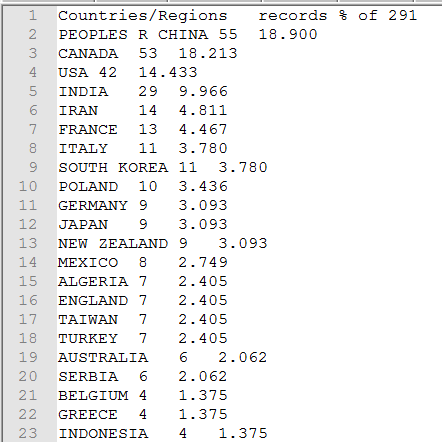
\includegraphics[width=9.5cm,height=4cm]{images/Nliq1.png}}
\vspace{1em}
\item Country Wise Citation report for a university 
 
 \vspace{2em}
\uncover{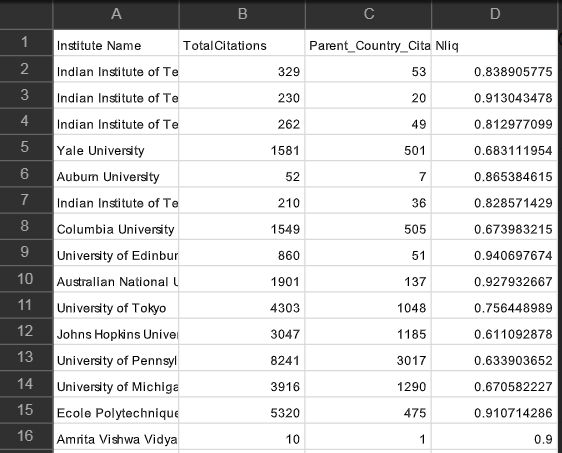
\includegraphics[width=9.5cm,height=4cm]{images/nliq2.png}}
\vspace{1em}
\item Calculated Nliq values with respective Institutions

\subsection{International Collaboration Ratio(ICR)}

The international Collaboration Ratio (ICR) is a novel metric that quantifies the extent to which each university collaborates with international collaborators. For each university, ICR can be broadly defined as the ratio between the weighted sum of the contributions of domestic authors and the weighted sum of the contributions of international collaborators.

%---------------------------------------------------

\subsection{Calculation of ICR}
        \item ICR calculation requires the following fields for each paper for each university.
        \begin{itemize}
  \item Number of authors who have authored the paper
  \item Number of authors belonging to different countries grouped by countries. Eg. 2 authors from India and 4 authors from USA.
  \item (Optional) Number of authors belonging to the same countries but different universities grouped by university. Eg. Out of 4 authors from India be 3 belong to PES and 1 belong to IISc.
\end{itemize}
      \begin{center}
         \uncover{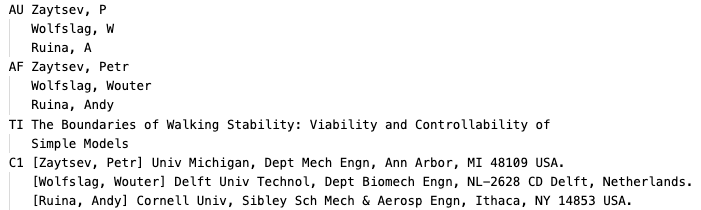
\includegraphics[scale=0.35]{images/data-sample.png}}
          {\tiny \item Sample data: A single paper from Cornell University}
    \end{center}




\subsection{ICR Algorithm}
\begin{enumerate}
        \item Calculate the weight of each article belonging to each institution as follows
        
              \begin{center}
         \begin{equation*}
Weight = \frac{\frac{No.\ of\ different\ collaborating\ countries\ for\ article}{Total\ no.\ of\ authors}}{ No.\ of\ authors\ from\ institution\ to\ which\ article\ belongs}
\end{equation*}
    \end{center}
    \vspace{1em}
\item Calculate ratio of normalised weights and the total number of articles from the university which are written with International Collaboration 
\begin{center}
         \begin{equation*}
ICR = \frac{\sum^{}Normalised\ Weights}{Total\ no.\ of\ articles\ written\ with\ IC}
\end{equation*}
    \end{center}
\end{enumerate}
       
\subsection{ICR Calculation Example}
\item If an article has 5 authors where 2 authors from India, 3 from USA (2 from same institution in USA, 1 from different institution in USA)
\begin{itemize}
        \item For Indian institution, weight of article will be
        
              \begin{center}
         \begin{equation*}
Weight, W1 = \frac{\frac{2}{5}}{2} \ and 
\ Normalised\ weight, NW1 = \frac{W1}{5}
\end{equation*}
    \end{center}
     \item For institutions from USA, weight of articles will be
        
              \begin{center}
         \begin{equation*}
Weight, W2 = \frac{\frac{2}{5}}{2} + \frac{\frac{2}{5}}{1} \ and 
\ Normalised\ weight, NW2 = \frac{W2}{5}
\end{equation*}
    \end{center}
    
\item ICR calculation
\begin{center}
         \begin{equation*}
ICR = \frac{\sum^{}(NW1,\ NW2)}{1} = 0.16
\end{equation*}
    \end{center}
\end{itemize}
       
       
\section{Implementation using PSO}
We have used PSO to find the value of $\rho$ at which the output,Q of the CES function is maximum. 
    PSO is a computational method that optimizes a problem by iteratively trying to improve a candidate solution with regard to a given measure of quality.
    
    
\subsection{PSO algorithm}
\begin{algorithm}[H]
\caption{Particle Swarm Optimization Algorithm}
    \KwResult{1) Position and velocity of particles at which cost is optimal 2) Optimum cost}
  \begin{algorithmic}[1]
  \STATE Initialize an array of particles with random positions [x1,x2,x3,....] and velocities [v1,v2,v3....] on d dimensions in the problem space
  \WHILE{stopping condition is not met}
   \STATE Evaluate the objective function, (in our case the CES function) for each particle
    \IF{current particle’s fittness is better than the previous best, ’pbest’}
      \STATE current particles best is saved as the ’pbest’ and the ’pbest’ location corresponds to thecurrent location in D-dimensional space.
    \ENDIF
   \STATE Compare Pbest of particles with each other and update the swarm global best location with the greatest fitness (gbest).
   \STATE Modify the velocity and position of the particles according to the following equation
  \begin{equation}
      v[i+1] = w*v[i] + c1*rand1*(pbest-x[i]) + c2*rand2*(gbest-x[i])
  \end{equation}
    \begin{equation}
      x[i+1] = x[i]+v[i+1]
  \end{equation}
  \ENDWHILE
  \RETURN best position and cost.
  \end{algorithmic}
\end{algorithm}

  
\subsection{PSO Python pseudocode}
We have implemented our proposed model using the Particle Swarm Algorithm (PSO).  
\begin{lstlisting}[language=Python]
# Import pyswarm package for PSO implementation
import pyswarms as ps
import math
import pandas as pd
import numpy as np

# Load dataset
df = pd.read_csv('data/icr-nliq-combined.csv')
df = df.fillna(0)

# Define constraints for rho
max_bound = 1.0 * np.ones(1)
min_bound = 0 * np.ones(1)
bounds = (min_bound,max_bound)

# Define options for PSO
#
#v[i+1] = w*v[i] + c1*rand1*(pbest-x[i]) + c2*rand2*(gbest-x[i])#
#
# Define variables c1,c2 and w for the above PSO equation
options = {'c1': 0.6, 'c2': 0.3, 'w': 0.9}

#Run PSO Iteratively for each record in the dataset 

internationality = []
rho = []
K =[]
L=[]
for d in range(len(df))[:]:
    q.setparams(K=df['ICR'][d],L=df['NLIQ'][d])
    print(q.K,q.L)

    # Set-up optimizer
    optimizer = ps.single.GlobalBestPSO(n_particles=25, dimensions=1, options=options,bounds =bounds)
    # Function f is the CES function which takes outputs the internationality score Q. 
    inter,r = optimizer.optimize(f, iters=100)
    print('internationality: %f\Rho%f'%(inter,r))
    # Plot the internationality
    internationality.append(inter)
    rho.append(r[0])

# Append to dataframe
df['internationality'] = internationality
df['rho'] =rho
\end{lstlisting}

\newpage
\section{Results}
\begin{figure}[h]
    \centering
    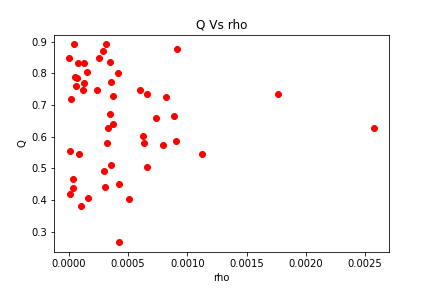
\includegraphics[scale=0.4]{images/qVSrho.png}
    \caption{The above graph is a scatter plot of the internationality, Q VS elaticity $\rho$. Each point on the graph represents a separate institution.}
    \label{fig:my_label}
\end{figure}

\subsection{PSO learning curve}

The below graph shows a trace of the cost history duting PSO optimization. It is the learning curve when K(ICR) = 0.01 and L(NLIQ) = 0.666666667. The values of $\rho$ and internationality (cost) at the global optima is: \\$rho$=0.4382448117430233 and  \\internationality=0.00057745 

\begin{figure}
\begin{subfigure}{.5\textwidth}
  \centering
  % include first image
  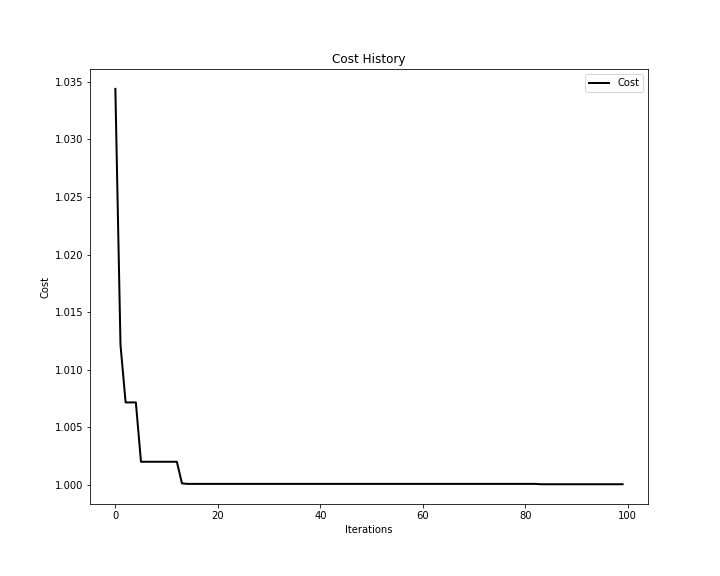
\includegraphics[width=.7\linewidth]{images/cost.png}  
  \caption{}
  \label{fig:sub-first}
\end{subfigure}
\hfill
\begin{subfigure}{.5\textwidth}
  \centering
  % include second image
  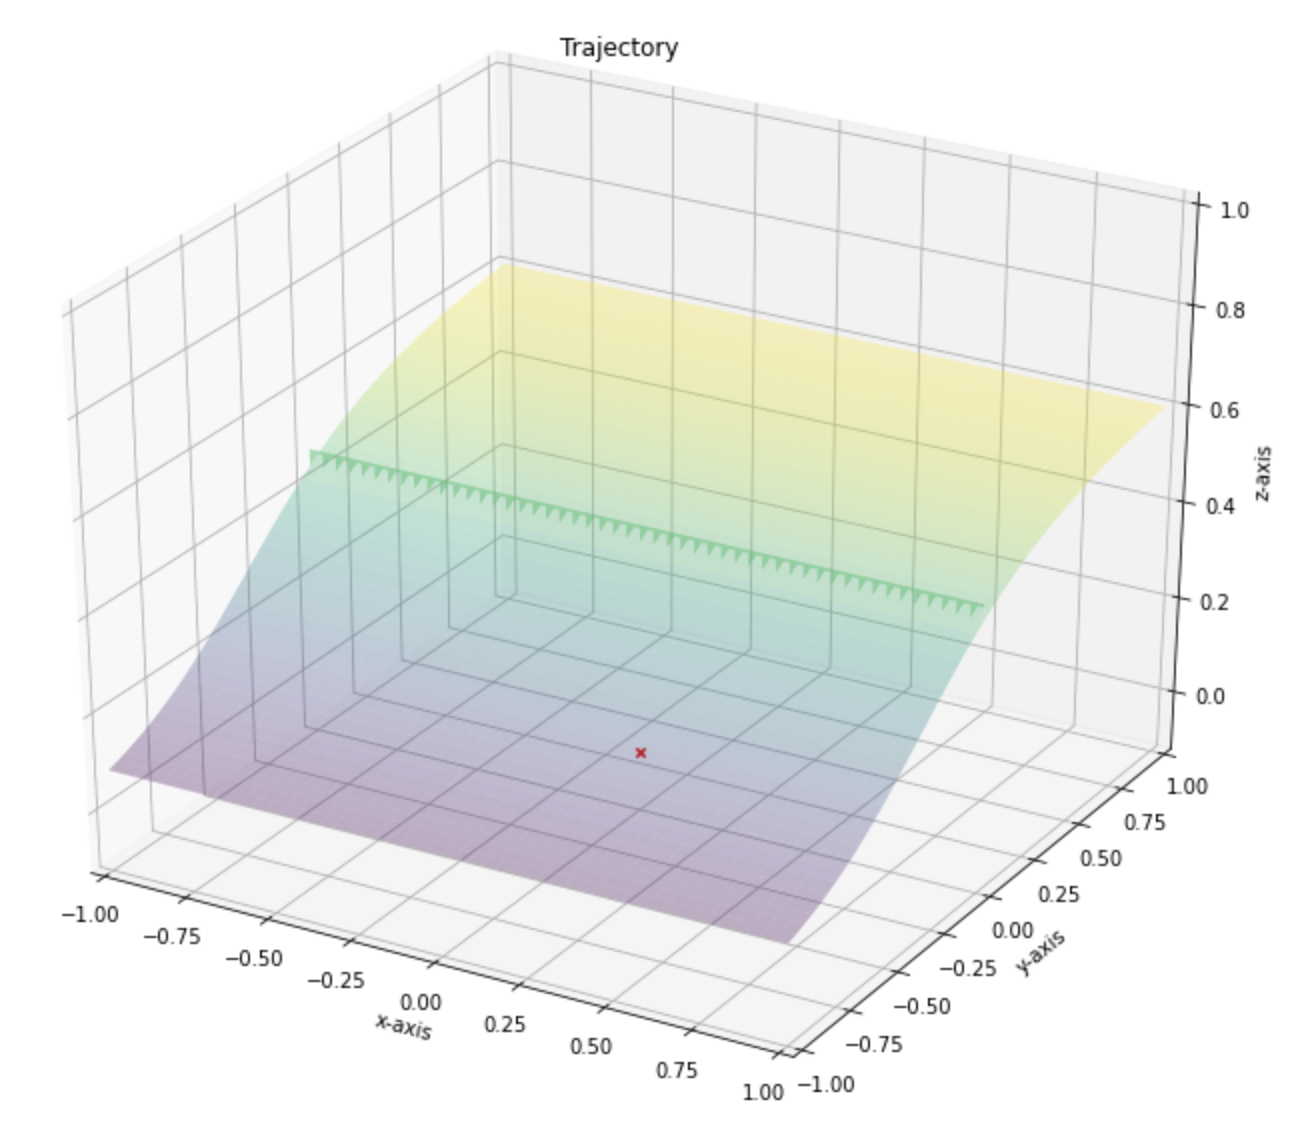
\includegraphics[width=.7\linewidth]{images/cost_opt.png}  
  \caption{}
  \label{fig:sub-second}
\end{subfigure}
\caption{Learning curve for PSO optimization}
\label{fig:fig}
\end{figure}


\subsection{Result for constrained PSO optimization}
\newpage
We compare the different values of rho obtained after restricting the values of $\rho$ between different intervals 1) 0.0-1.1 2) 0.001-0.1 
3) 0.101-0.9 
4) 0.9-0.99 
5) >1  \\
This table below shows the internationality scores of each institute calculated based on the fixed NLIQ and ICR values and the optimized elasticity, $\rho$ values. The results are arranged in the decreasing order of their internationality score.

\begin{table}[ht!]
    \centering
    \begin{tabular}{ | m{15em} | m{1cm}| m{1cm} |m{1cm}| m{1cm}|m{1cm}| m{1cm}| m{1cm}|} 
\hline
Institution & ICR & NLIQ & 0-1 & 0.001-0.1 & 0.101-0.9 & 0.9-0.99 & >1\\ 
\hline
University of Southern Queensland & 0.75 & 0.90 & 0.8917 &	0.8917 &	0.89191 &	0.8930 & 0.0 \\ 
\hline
Alexandria University & 0.5833&	0.9348 &0.8917 &0.8917 &	0.8926 &	0.8989 &0.0\\
\hline
Auburn University & 1.0	& 0.8653 & 0.8779 &	0.8780 &	0.8781 &	0.8788 &	0.9981\\
\hline 
Australian National University & 0.4929 & 0.9279 & 0.8711 &	0.8711 &	0.8726 &	0.8833 & 0.0\\
\hline
IISC - Bangalore &
 0.8571 &	0.8486 & 0.8494 &	0.8494 &	0.8494 & 0.8494 &	0.0\\
\hline
BITS Pilani & 0.3333 &	0.94  & 0.8474 &	0.8475 &	0.8515 &	0.8769	& 0.0\\
\hline
\end{tabular}

    \caption{Cost i.e Q(Internationality)  values for each institute for 6 different ranges pf $\rho$. This table shows the NILQ, ICR and cost values for the first 5 universities. The value of alpha=0.1}
    \label{tab:al_0.1}
\end{table}

\begin{table}[h]
    \centering
    \begin{tabular}{ | m{15em} | m{1cm}| m{1cm} |m{1cm}| m{1cm}|m{1cm}| m{1cm}| m{1cm}|} 
\hline
Institution & ICR & NLIQ & 0-1 & 0.001-0.1 & 0.101-0.9 & 0.9-0.99 & >1\\ 
\hline
Auburn University & 1.0	& 0.8653 & 0.9303 &	0.9303 &	0.9305 &	0.9324 &	0.9992\\
\hline
IISC - Bangalore &
 0.8571 &	0.8486 & 0.8528 &	0.8528 &	0.8528 &	0.8528 &	0.0\\
\hline 
University of Southern Queensland & 0.75 & 0.90 & 0.8257 & 0.8257 &	0.8261 & 0.8291 	& 0.0 \\ 
\hline
Alexandria University & 0.5833&	0.9348 & 0.7384 &	0.7385 & 0.7405 &	0.7570 &	0.0\\
\hline
\end{tabular}

    \caption{Cost i.e Q(Internationality)  values for each institute for 4 different ranges pf $\rho$. This table shows the NILQ, ICR and cost values for the first 5 universities. The value of alpha=0.5}
    \label{tab:al_0.5}
\end{table}

Table \ref{tab:al_0.1}
shows the ranking of institutions after executing PSO for the following ranges of $\rho$; 1) 0.0-1.1 2) 0.001-0.1 
3) 0.101-0.9 
4) 0.9-0.99 
5) >1. %The ranked output of 1,0000 candidates is available in [4].
Apparently, results for all conditions are consistent and it can be noticed that the ranking results are same for most of the institutes till  $rho<0.9$. This shows that the model works in harmony for all ranges of $\rho$ between 0 and 1. Also, score is at higher side for candidates that have high NLIQ and ICR. Evidently the model gives more weightage to lineage independent parameters while computing scores, and brings out candidates with larger NLIQ and ICR at higher positions if these values are large. \\
Table \ref{tab:al_0.5} shows the ranking of the institutions when $\alpha$ is set to 0.5. We can see that the ranking slightly changes as equal weight is given to both ICR and NLIQ. For example Auburn university which has ICR=1 and NLIQ=0.86 is ranked 1 when $\alpha=0.5$ but when $\alpha=0.1$, University of Southern Queensland is ranked first. This shows that when $\alpha=0.1$, institutions with larger values of NLIQ is ranked higher, but when $\alpha=0.5$ equal weightage is given to both ICR and NLIQ.

%Figure  are plots that demonstrate the change in the CES function with respect to the values of $\rho$. The plots are drawn for top-three ranked candidates.


%\begin{figure}[h]
 %   \centering
 %   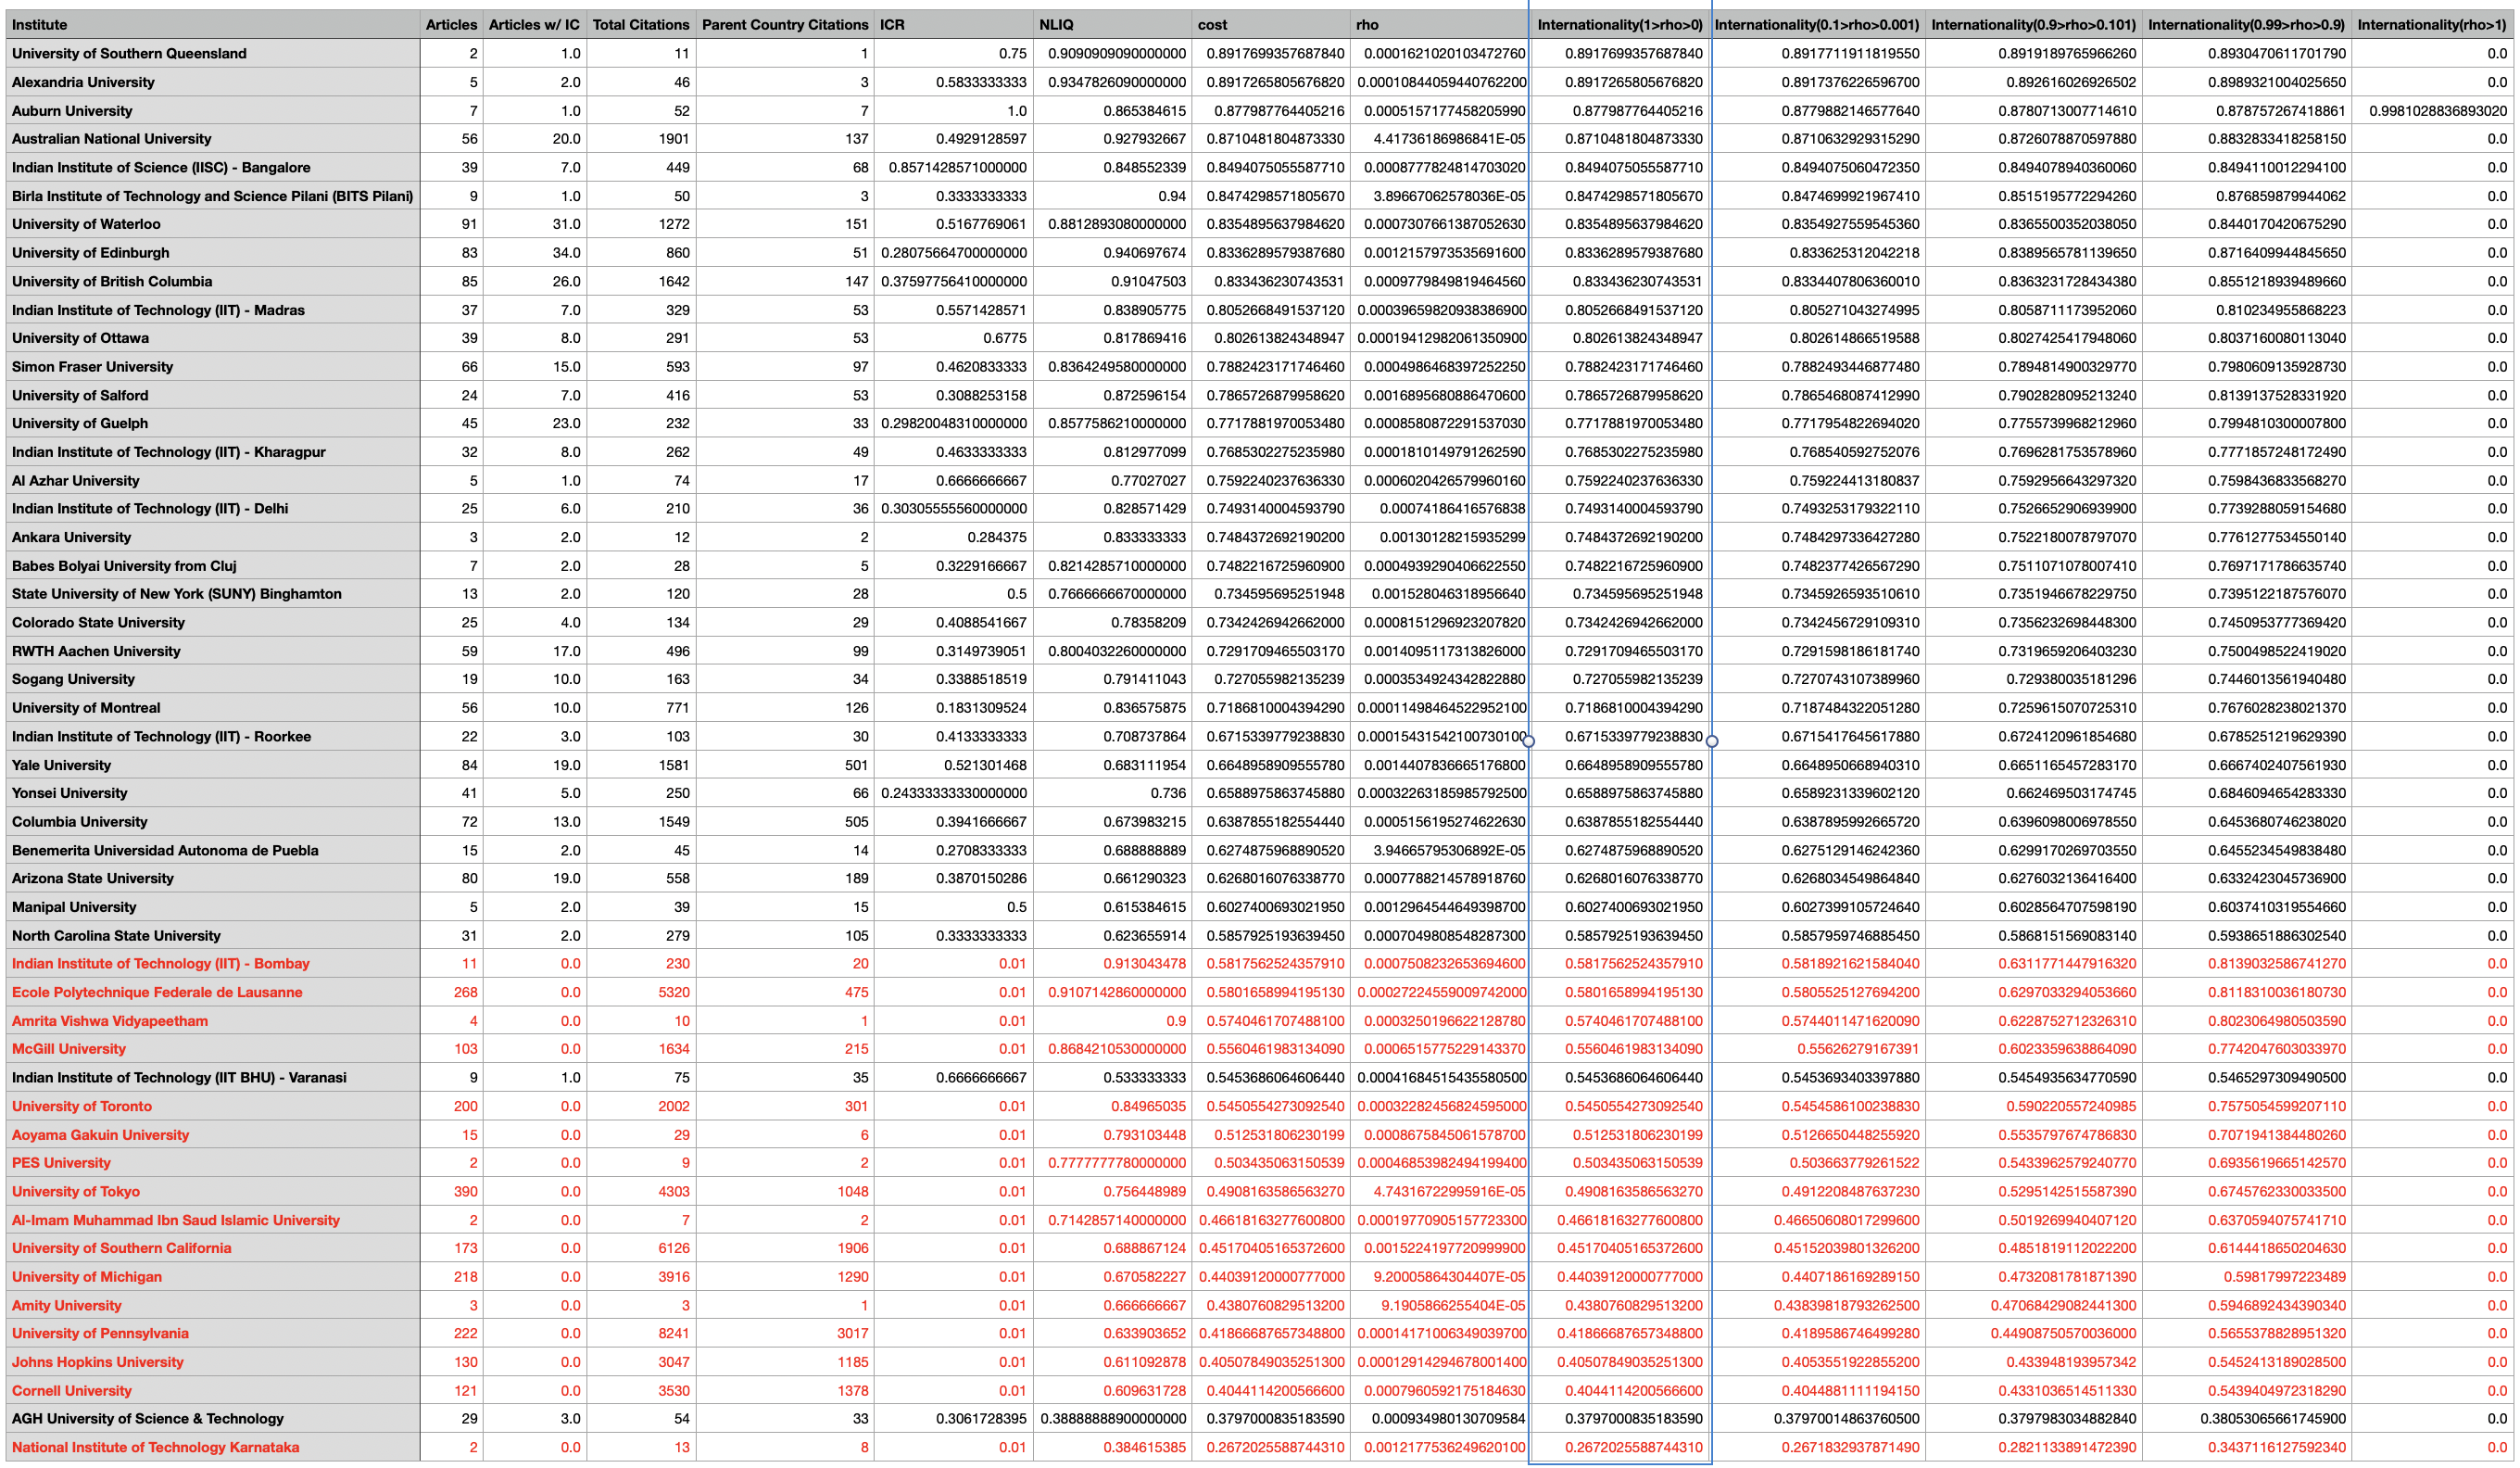
\includegraphics[scale =0.35]{images/pso_res.png}
 %   \caption{Cost i.e Q(Internationality) and $\rho$ values for each institute. This table shows the $\rho$ and cost values for the first 20 universities.}
%    \label{fig:my_label}
%\end{figure}


%\subsection{Interpretation of result}
\\
  
\begin{table}[h]
    \centering
\begin{tabular}{ | m{15em} | m{1cm}| m{1cm} |m{1cm}| m{1cm}|m{1cm}| m{1cm}| m{1cm}|} 
\hline
Institution & ICR & NLIQ & 0-1 & 0.001-0.1 & 0.101-0.9 & 0.9-0.99 & >1\\ 
\hline
Indian Institute of Technology (IIT) - Kharagpur & 0.46333 &	0.8129 & 0.7685	& 0.7685 &	0.7696 &	0.7772 & 0.0 \\ 
\hline
Simon Fraser University & 0.4620 &	0.8364 & 0.7882 &	0.7882 &	0.7895 & 0.7981	& 0.0\\
\hline
\end{tabular}
    \caption{Comparison between 2 universities having similar NLIQ and ICR values.}
    \label{tab:comptab}
\end{table}

Table \ref{tab:comptab} shows 2 universities having comparable NLIQ and ICR values; Simon Fraser University and IIT-Kharagpur. We see that the value of rho and internationality varies although the NLIQ and ICR values are very similar. This is at par with our initial hypothesis, where we considered this system modelled using CES to be chaotic in nature.  
%\begin{figure}[ht!]
%    \centering
%    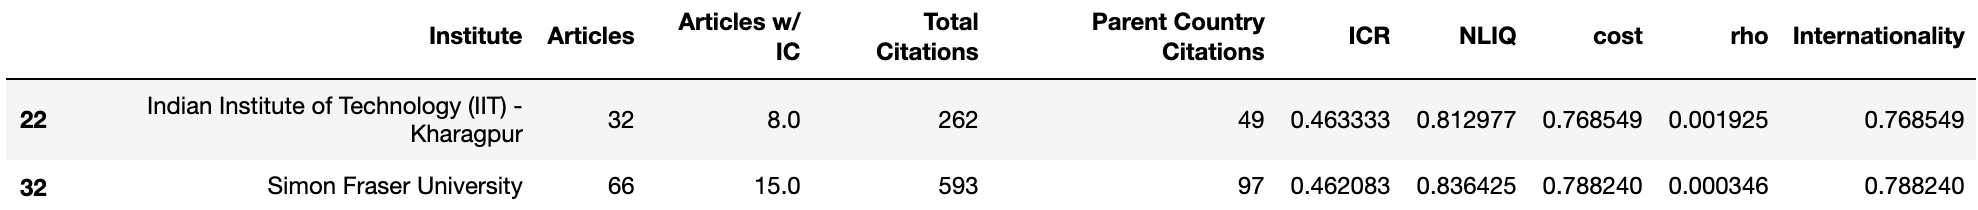
\includegraphics[scale = 0.5]{images/sim_uni_comp.png}
%    \caption{Comparison between 2 universities having similar NLIQ and ICR values.}
%    \label{fig:my_label}
%\end{figure}


\newpage
\subsection{Plotting output of production function of different values of $\rho$}
Traditional approaches are aimed at varying K and L input factors and monitoring the variation of output with changing input factors such as an increase in ICR or NLIQ. However, in economic models, the output of a system can also change due to unexplainable random events, popularly known as the superstar effect. The Superstar Effect refers to the change in performance caused by the presence of a highly ranked player - a superstar - in a rank-order competition. In the CES equation this super star effect is captured by the elasticity variable $\rho$. In the above figure we plot the rate of change of output as well as the output with respect to the elasticity, $\rho$. We can observe that the rate of change of output increases with changing elasticity. Moreover, the output itself also increases with increase in elasticity.\\


\begin{figure}[h]
    \centering
    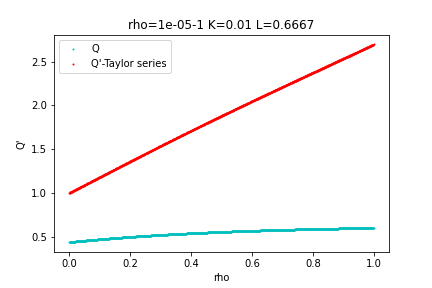
\includegraphics[scale=0.5]{images/0.01-0.67.png}
    \caption{The above figure shows how the internationality (Q) varies with $\rho$. $\alpha=0.1$}
    \label{fig:my_label}
\end{figure}

We are trying to find the rate of change output with respect to the an unknown factor(unexplainable value) $\rho$. $\rho$ signifies an unknown factor that could cause an increase in the output Q.


\begin{figure}[htpb]
\centering
\begin{subfigure}{0.45\textwidth}
\centering
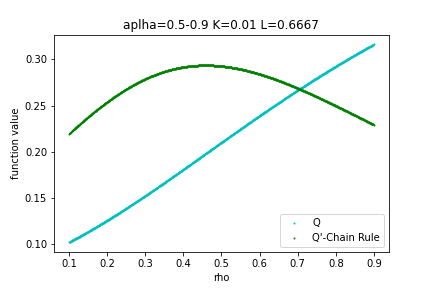
\includegraphics[width=\linewidth]{images/graphs/Q1_chain_0.101_0.9_alpha_0.5.png}
\caption{Function Value v/s $\rho$(0.0 \textless $\rho$ \textless 0.1)}
\end{subfigure}
\begin{subfigure}{0.45\textwidth}
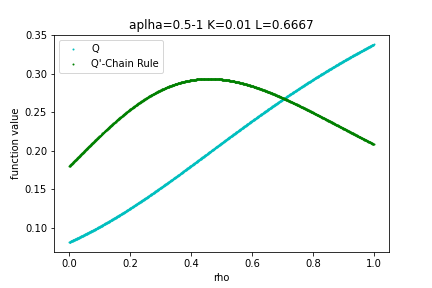
\includegraphics[width=\linewidth]{images/graphs/Q1_chain_alpha_0.5.png}
\caption{[Function value v/s $\rho$ (0.1 \textless $\rho$ \textless 0.99]}
\end{subfigure}
\caption{Plots to see how CES function changes with the values of $\rho$. Function v/s $\rho$ is plotted for K=0.01 and L=0.6667. This is evident from the plots that, as value of $\rho$ changes, it attains an optimum value. }
\label{fig:test3}
\end{figure}


\begin{figure}[H]
  \centering
  \begin{subfigure}{0.450\textwidth}
    \centering
    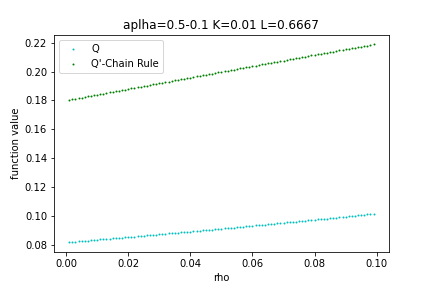
\includegraphics[width=\linewidth]{images/graphs/Q1_chain_0.001_0.1_alpha_0.5.png}
    \caption{Function value v/s $\rho$ (0.0 \textless $\rho$ \textless 1)}
 
  \end{subfigure}
  \begin{subfigure}{0.450\textwidth}
    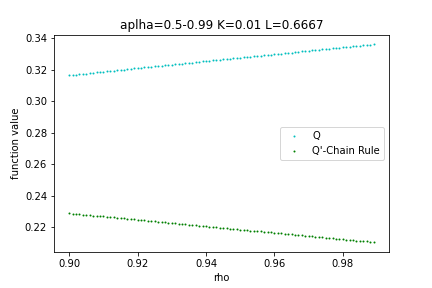
\includegraphics[width=\linewidth]{images/graphs/Q1_chain_0.9_0.99_alpha_0.5.png}
\caption{Function value v/s $\rho$ (0.1 \textless $\rho$ \textless 0.99)}
    
  \end{subfigure}
  \caption{Plots to see how CES function changes with the values of $\rho$. Function v/s $\rho$ is plotted for K=0.01 and L=0.6667. This is evident from the plots that, as the value of $\rho$ changes, it attains an optimum value.}.
  \label{fig:test2}
  \end{figure}


\end{document}
